\documentclass[a4paper,10pt]{report}
\usepackage[utf8]{inputenc}
\usepackage{graphicx}
\usepackage{float}
\usepackage{amsmath}
\usepackage{amssymb}
\usepackage{listings}


\setlength{\parindent}{0pt}

% Title Page
\title{Trees}
\author{Zack Garza}


\begin{document}
\maketitle

\begin{abstract}
\tableofcontents
\end{abstract}

% Definitions, history, statement of the main results, proofs, applications, open questions
%Why is the problem you are solving worth solving?
% What is the core difference between your method and all those that came before? This is really a two-part question (which most speakers screw up by answering only the second part).
% What does your method accomplish that no previous method accomplishes?
% What algorithmic or methodological idea enables your method to accomplish more?
% What is the evidence that your method is better in some circumstances? (And what are those circumstances?)
% What is the one big idea that you want people to leave your talk with? If you try to get across five ideas, you will usually impart none. If you choose one main idea and focus on advertising it, you will usually succeed. “Give them something to take home.”
\chapter{Background and Definitions}

\subsection{Background}
So, today I'm going to talk to you guys about trees, and hopefully give you guys some insight into why they're a particularly nice object to work with.

\begin{itemize}

\item To start off, we won't actually define a tree at first, but we'll talk a bit about why they were ``invented'' in order to address the question of why we would  need something like a tree in the first place.

\item Then, we'll talk about what a tree really is, plus when and where they might be useful.

\item Then we'll go over a few of the interesting properties that trees have, as well as a few different variants of them.

\item And lastly, we'll cover some of the ways trees can be applied to problems.\\
\end{itemize}

So first, for a little bit of background -- trees were first studied in the late 1800s by Arthur Cayley, who made contributions to geometry and analysis. For those of you that might go on to take further courses in math, you'll very likely come across Cayley's Theorem in a class that covers groups (which is a topic in abstract algebra). You'll spend a lot of time studying things called ``permutation groups'', and Cayley's Theorem showed that theorems which were true for permutation groups could be extended to be true for all groups in general.\\

Much of Cayley's work revolved around studying which properties of objects were invariant under some condition -- that is, after applying some kind of transformation to the object, the property remained the same and was in a somehow fundamental to that object's structure.\\

For example, consider rotating a circle in the plane -- this does not change the set of points contained within the circle. Or consider switching rows and columns of a matrix -- the set of elements inside of the matrix is the same.\\

So where do trees come into this? Well, Cayley invented trees while working with chemical structures -- in particular, he was trying to find a way to mathematically generate the structure of hydrocarbons. (See Figure).\\

\begin{figure}[h!]
	\begin{centering}
	\begin{center}
	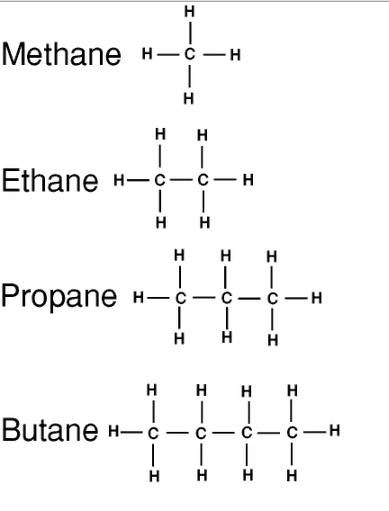
\includegraphics[width=\linewidth]{./Pictures/alkanes.png}
	\caption{A series of Alkanes -  one $C$ always bonds to 4 other atoms, and the structure always conforms to the relationship $H_n-C_{2n+2}$}
	\label{fig:alkanes}
	\end{center}
	\par\end{centering}
\end{figure}

\begin{figure}[H]
	\begin{centering}
	\begin{center}
	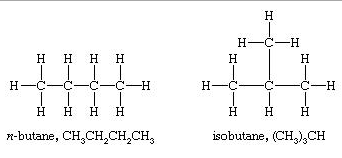
\includegraphics[width=\linewidth]{./Pictures/hydrocarbons.png}
	\caption{Applying a transformation (in this case, relocating a bond to create an isomer) does not affect the number of $H$ and $C$ atoms, but can change the ways in which they bond.}
	\label{fig:hydrocarbons}
	\end{center}
	\par\end{centering}
\end{figure}

One thing to notice about the alkane series above is that for $n\leq 3$, no matter how we many ways we ``swap'' the atoms, we can always find a way to make our 'swapped`` version look like one of the given versions. But for $n \geq 4$, something interesting happens -- now, we have a way of swapping atoms that really has changed the structure. And if you're doing chemistry with these compounds, this is something you might worry about -- although the number of $H$ and $C$ atoms is the same, we know that these kinds of structural changes can cause the chemical to react in an entirely different way!\\

In chemistry, we might call these two forms ''isomers``, but Cayley's observation was that something more general was going on. If these could be formulate as mathematical objects, then it might be said that isobutane was a permutation that wasn't \textit{isomorphic} to the rest of the permutations on 4 atoms. And hydrocarbon chains can easily extend into 100s of atoms - then what could we say about an an arbitrary set of $n$ atoms? And is there a function that could generate these kinds of structures?

Well, it turned out that by abstracting some of the details way and dealing with these as mathematical objects, it became possible to begin finding answers to these questions.

\subsection{Motivation}
So what kinds of things are trees useful for?

Used widely in computer science

\begin{enumerate}
	\item Game state trees (checkers, chess, etc.) - vertices represent states, and edges represent valid moves. (See Figure)
	\item Huffman encoding - Given a large amount of text, it can be compressed into a tree based on symbol frequency. Used in jpeg, mp3, and zip as an algorithm for lossless compression.
	\item Decision trees
	\item Efficient, structured storage - certain types of trees are guaranteed to be bounded by $O(\log n)$ (as long as they are balanced, as in certain B-trees or Red-Black trees.)
	\item Form the basis of heaps, which are used to implement priority queues. These are used for operating system scheduling processes, quality-of-service in routers, AI path-finding algorithms, etc.
\end{enumerate}

Most things that can be represented in a hierarchy can be modeled as trees. From a practical perspective, they are also very easy to implement. They can be defined recursively, and have no theoretical upper limit to the amount of vertices. They are also amenable to proofs by induction.

What are trees not so good for?
Generally, any graph that contains loops. For example, a circuit that could be represented as a tree would have no current.

\subsection{The Basics}
So we need to define what exactly we mean when we talk about trees. We'll have to go through a bunch of definitions first, so let's get to it!\\

A tree is a mathematical object that can be viewed as a graph, or computer scientists might classify it as an \textit{abstract data type} or ADT.\\

Tree are generally structured like this:
\begin{figure}[h!]
	\begin{centering}
	\begin{center}
	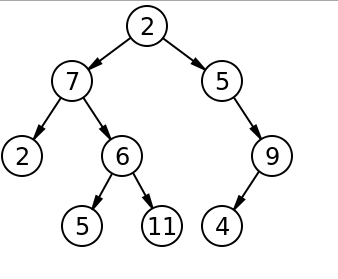
\includegraphics[width=\linewidth]{./Pictures/basic_tree.png}
	\caption{A basic tree.}
	\label{fig:basic_tree}
	\end{center}
	\par\end{centering}
\end{figure}

At a bare minimum, it consists of elements that we refer to as \textit{vertices} that are connected, and these connections are usually represented as paths or \textit{edges} between the vertices. The edges themselves can have additional structure, such as specifying a direction between vertices, or assigning a numerical value or \textit{weight} to each edge.\\

We also impose two other conditions, but we'll need a few definitions from graph theory to do so:\\

\textbf{Definition.} A graph $G(V,E)$ is a set of nodes and vertices.

\textbf{Definition.} Given a graph $G$, a path $(v_1, v_2, v_2, \cdot v_n)$ is called a \textit{cycle} if $v_1 = v_n$. A graph that does not contain a cycle is said to be \textit{acyclic}.

\hrulefill

\textbf{Definition.} A graph $G$ is called \textit{connected} if \underline{for every pair of vertices, $(v,w)$}, there exists a path between them.

\textbf{Definition:}  A graph $G$ is a tree if $G$ is \underline{connected} and \underline{acyclic}.

\hrulefill

Examples of Definitions:
%The similar problem of counting all the subtrees regardless of size has been shown to be #P-complete i
\begin{figure}[H]
	\begin{centering}
	\begin{center}
	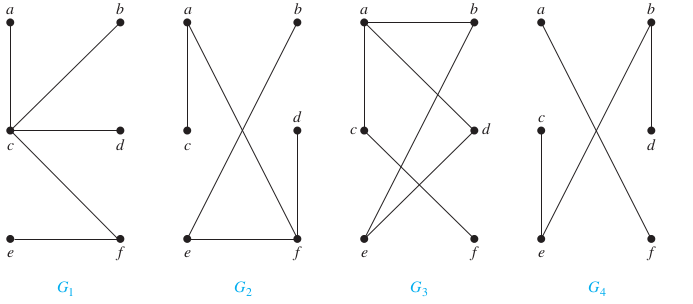
\includegraphics[width=\linewidth]{./Pictures/some_trees.png}
	\caption{A few undirected graphs; which are trees? $G_1$ and $G_2$ are, but $G_3$ contains a cycle and $G_4$ is not connected, but is a disjoint union of trees and is referred to as a \textit{forest}.}
	\label{fig:some_trees}
	\end{center}
	\par\end{centering}
\end{figure}

\newpage
How you would implement a Tree:
\begin{lstlisting}[language=C++]
class BSTree {
    struct node
    {
        Record r;
        *node[n] children;
    };
	node* root
}
\end{lstlisting}

Compare this to an implementation of a Linked List, and you'll see that they are very similar:
\begin{lstlisting}[language=C++]
class DLList {

    struct node
    {
	int data;
        node* next;
    };

    node* head;
    node* cursor;
\end{lstlisting}



And trees have an entire language associated with them, so we'll clarify a few definitions:
\begin{enumerate}
	\item Degree - the number of edges emanating from a node.
	\item Parent - If $v$ is a vertex, the parent $p$ is the unique vertex such that $p\Rightarrow v$.
	\item Child - If $p$ is the parent of $v$, $v$ is the child of $p$
	\item Sibling - Vertices with the same parent.
	\item Ancestor - Any vertex on a path between $v$ and the root.
	\item Descendant - Vertices for which $v$ is an ancestor.
	\item Internal Vertex - Any vertex with children.
	\item Leaf - Vertex with no children
	\item Subtree - Subgraph consisting of a node $v\in T$ as its root, including all of its descendants.
	\item Height - Number of edges along the longest path between a vertex and a leaf.
	i.e., a local measure of how far a vertex is from a leaf.

	Leaves are defined to have a level of 0.

	\item Depth - Number of edges between a vertex and the root vertex,
	i.e. a measure of distance to the root vertex.

	Root vertices are defined to have a depth of 0

		\begin{figure}[H]
		\begin{centering}
		\begin{center}
		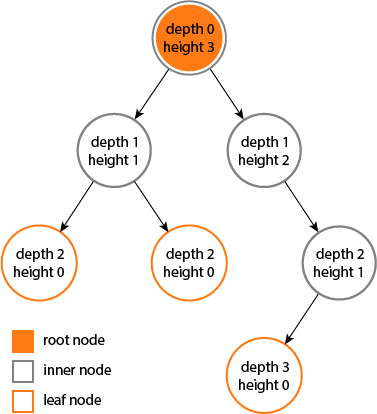
\includegraphics[width=.5\linewidth]{./Pictures/height-depth.png}
		\caption{Root vertices always have a \underline{depth} of 0, and leaf vertices will always have a \underline{height} of zero. }
		\label{fig:??????}
		\end{center}
		\par\end{centering}
		\end{figure}
\end{enumerate}


Alright, so now we can talk a little more precisely about trees -- but so what? What did we gain from this abstraction? Well, trees have some nice properties. In particular,
\begin{enumerate}
	\item Given two distinct vertices $u$ and $v$ in a tree, there exists a \textit{unique} path between them.
	\item If we cut or remove any edge of a tree, it is no longer a tree -- this guarantees that a tree is a \textit{minimally connected} graph.
	\item If a tree has $n$ vertices, then it has $n-1$ edges.
	\item Trees obey Euler's Polyhedra formula (which states that the vertices, faces, and edges of a 3-dimensional polyhedron obey the equation $V+F-E=2$. Considering the tree as a one-dimensional polygon, we get $V-E=1\rightarrow V=1+E$.)
\end{enumerate}


Of course, by giving trees a mathematical structure, we can formally prove these kinds of things! And so we shall!

\hrulefill

\noindent\textbf{Theorem: }An undirected graph is a tree iff there is a unique, simple path between any two vertices.

\textit{Proof:} For the theorem to hold, it must be shown that
\begin{itemize}
	\item If $T$ is a tree, then there is a unique simple path between every two vertices.
	\item If $G$ is an undirected graph with a unique, simple path between every two vertices, it is a tree.
\end{itemize}


\textbf{(1)} If $T$ is a tree, then there is a unique simple path between every two vertices.

\textit{Proof by contradiction:}\\

Assume we have a tree $T$.\\

Then by definition, it is a graph, and it must be connected and contain no simple circuits.\\

Pick two vertices, $u_0$ and $v_0$.\\

Because $T$ is connected, there will always exist a simple path $P_1:(u_0, u_1, u_2\cdots,v)$ between $u$ and $v$.\\

But from our assumption that $T$ is a tree, there can be no simple circuits - that is, there does not exist a path $P_n:(u_0, u_1, u_2\cdots,v,\cdots u_n)$ such that $u_n = u_0$.\\

Assume there was another path, $P_2$ -- if this path existed, it could be combined with $P_1$ and create $P_n$. This contradicts the conclusion that $P_n$ does not exist in $T$, which contradicts our assumption that $T$ was a tree.\\

\textit{So, by contradiction, if $T$ is a tree, then there is a unique simple path between every two vertices.} \\ \\

\textbf{(2)} If $G$ is an undirected graph with a unique, simple path between every two vertices, it is a tree. (We want to show $G$ satisfies the definitions of a tree). \\

\textbf{(2a)} $G$ is connected.\\
\textit{Direct Proof:}
Assume we have a graph $G$ such that for every two vertices $x_0$ and $y_0$, there exists a unique path $P_0:(x_0, x_1, x_2,\cdots y_0)$. \\

But this is simply our definition of a connected graph, so $G$ must be connected, and the first part of our definition of a tree is satisfied. \\

\textbf{(2b)} $G$ contains no cycles.\\

\textit{Proof by contradiction:}
Suppose $G$ did have a cyclic path $P_c:(x_0, x_1, x_2,\cdots,y_0,\cdots,x_n)$ such that $x_n = x_0$.

This implies that there are at least two simple paths between $x$ and $y$:

$P_{c1}:(x_0, x_1, x_2,\cdots,y_0,)$ and
$P_{c2}:(x_n, x_{n-1}, x_{n-2},\cdots,y_0)$.

But this contradicts our assumption $P_0$ was unique.

\textit{So, by contradiction $G$ is connected and contains no simple circuits, and $G$ is by definition tree.}

\hrulefill






A useful consequence of this theorem is that the number of edges and vertices in a tree are always related:

\textbf{Theorem:} A tree with $n$ vertices has $n-1$ edges, where $n\in\mathbb{N}$.

\textit{Proof: }We utilize choice in this proof to distinguish vertices and pick an arbitrary root for the tree, and then proceed by induction. \\

Let $P_n$ be the statement of the theorem.

\textit{Basis: }
When $n=1$, $P_1$ states that a tree with 1 vertex has 0 edges, which is trivially true. \\

\textit{Induction: }
Assume $P_n$. Then, $P_{n+1}$ states that a tree with $n+1$ vertices has $n$ edges.

Consider such a tree, $T$. Since $T$ is finite, it must have a leaf. Remove this leaf to produce a tree $T'$, which must still be a tree because it remains connected and contains no simple circuits.

Since $T'$ now has $n$ vertices, by the inductive hypothesis, it then has $n-1$ vertices.

Adding one vertex requires adding one edge, which acts on $T'$ to transform it back to $T$, which must have $n+1$ vertices and $n$ edges.

\textbf{Thus, by mathematical induction $P_n$ is true for all $n$.}

\hrulefill

\chapter{Rooted Trees}
In practice, when we talk about and use trees, we give them a little more structure. Using the axiom of choice, we arbitrarily designate one node as the \textit{root}.

\textbf{Definition:} A \textit{rooted tree} is a tree in which one vertex is designated as the root, and every edge is directed away from the root.\\ \\

This means that there is no predefined notion of what the root is, as long as there is consistency in direction. (See Figure)


Harking back to the problems that motivated our discussion of trees, let's say you and I both reach into our mystical bag of set elements and pull out two trees, arbitrarily choosing a root. How can we know if we are talking about the same object or not? We alleviate this problem by introducing the next definition:\\

\textbf{Definition: } Two trees $T$ and $T'$ are said to be \textit{isomorphic} if there is a bijection $f:T\mapsto T'$ such that $(u,v)$ is an edge in $T$ iff $(f(u), f(v))$ is an edge in $T'$. We call the map $f$ an $isomorphism$ and write $T\simeq T'$.\\ \\

So what does this definition really mean? This just says that as long as the transformation you apply to my tree $T$ preserves the connections between any two vertices, you and I are really talking about the same tree. In fact, the map $f$ an \textit{equivalence relation} on trees, but I'll leave that as an exercise for you guys.\\

Fun fact; The problem of testing whether two trees with $n$ vertices are isomorphic is NP-Hard!\\

A quick refresher on complexity classes:

\textit{Note: In a deterministic Turing machine, the set of rules prescribes at most one action to be performed for any given situation. A non-deterministic Turing machine (NTM) may have a set of rules that prescribes more than one action for a given situation.}

\begin{enumerate}
	\item P: Running time can be bounded by a polynomial.
	\item NP: Solutions are easy to verify, but difficult to generate. (Does $7\times3=21$?)
	\item NP-Hard: The tipping scale -- finding a solution guarantees solutions to all NP problems, proving a solution doesn't exist guarantees no solutions to all NP problems. (If $x\times y$=23, what are $x$ and $y$?)
	\item NP-Complete: Both NP and NP-Hard.
\end{enumerate}



\subsection{m-ary Trees}

\textbf{Definition: } A rooted tree is called an \textit{m-ary tree} is every \underline{internal} vertex has at most $m$ children, and is said to be \textit{full} if every internal vertex has exactly $m$ children.

Note that the definition of full only applies to \textit{internal} vertices! If we counted leaves, no finite tree would ever fit this definition.

\begin{figure}[h!]
	\begin{centering}
	\begin{center}
	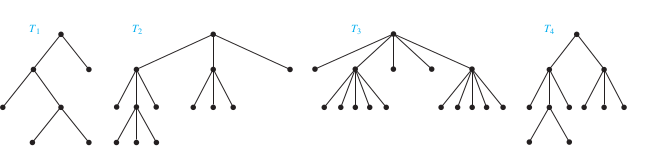
\includegraphics[width=\linewidth]{./Pictures/m_ary_exercise.png}
	\caption{Are these trees full $m$-ary trees from some $m\in\mathbb{N}$?}
	%If not, how can they be fixed? T4 just needs a third vertex added.
	\label{fig:??????}
	\end{center}
	\par\end{centering}
\end{figure}

\subsection{Special Case: Ordered Binary Trees}

We may also equip an $m$-ary tree with a \textit{partial ordering}, defined by the binary relation $v\leq w$ if $v$ is on a path between the root and $w$. Notice that this doesn't define a total ordering, as we haven't defined a way to compare sibling nodes. But this does have the added benefit of making the root a \textit{minimal element} of the tree.

Defined as an $m$-ary tree with $m=2$, i.e. that every vertex has two children. There is also an additional restriction that for a vertex $v$, all vertices in its left subtree are less than $v$, and all vertices in its right subtree are greater than $v$. Notice that now we have a \textit{total ordering} on the trees elements.

These are commonly used as data structures, and have several nice properties.

\textbf{Definition: }An $m$-ary tree  is \textit{complete} if every level (but not necessarily the last) is full, and all vertices on the bottom are on the left.

\begin{figure}[H]
	\begin{centering}
	\begin{center}
	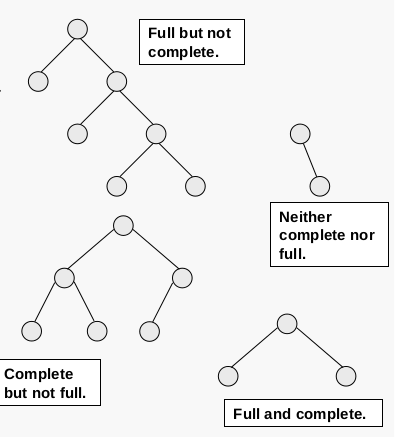
\includegraphics[width=\linewidth]{./Pictures/full_complete.png}
	\caption{Distinction between full and complete m-ary trees (in this case, binary).}
	\label{fig:??????}
	\end{center}
	\par\end{centering}
\end{figure}

\begin{figure}[H]
	\begin{centering}
	\begin{center}
	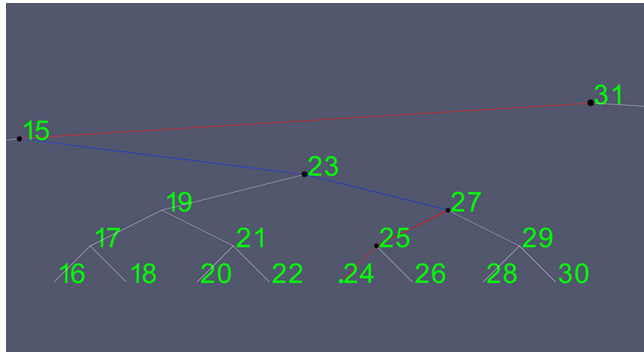
\includegraphics[width=\linewidth]{./Pictures/binary_tree_search.png}
	\caption{Binary trees can provide $O(\log n)$ access to arbitrary elements.}
	\label{fig:??????}
	\end{center}
	\par\end{centering}
\end{figure}

\textit{Big 'O' notation review:}
\textbf{Definition:} Let $f,g \in \mathbb{C}^{1}(\mathbb{R})$ . We say $f\in \mathcal{O}(g)$, or that $f$ is asymptotically bounded by $g$, if there exists a constant $\epsilon>0$ such that $f(n)\leq cg(n)$. (The constants $\epsilon$ and $c$ are sometimes referred to as a \textit{witness pair}. \\

Example: We might denote the error in an approximation as such:
\begin{align*}
	e^x = \frac{1}{2}(1+x+x^2) + \mathcal{O}(x^3).
\end{align*}


How do we know that lookup can be done in $O(\log n)$?

\textbf{Proof}

Well, suppose we have a full and complete binary tree $B$, with a maximum depth of $d$, and $n$ vertices.

To find an arbitrary vertex in $B$, we need to make at most $d$ comparisons -- one at each level of the tree.

But how is this related to the number of vertices in the tree?
Well, we count the vertices and see that
\begin{align*}
	n \leq 1 + 2 + 4 + 8 + \cdots + 2^d = \sum_{k=0}^d (1)2^k =(1)\frac{1-2^{d-1}}{1-2} = 2^{d-1} -1 \\
	\Rightarrow n \leq 2^{d-1} -1.
\end{align*}

That is, that the maximum number of vertices in a tree is bounded by the depth in a particular way. Solving for $d$, which the maximum number of comparisons needed, we see that

\begin{align*}
	&n+1 \leq 2^{d-1}  \\
	&\Rightarrow \ln(n+1) \leq (d-1)\ln 2  &\qquad\text{(where $\ln x$ is monotone increasing)} \\
	&\Rightarrow \lceil \frac{\ln(n+1)}{\ln 2}\rceil \geq d-1 &\qquad (\text{where }\ln 2 < 0) \\
	&\Rightarrow \lceil \log_2(n+1)\rceil+1 \geq d  &\qquad (\text{where $log_a(x) = \frac{log_b(x)}{log_b(a)}$})\\
	&\Rightarrow d \leq \lceil\log_2(n+1)\rceil +1 \leq c\log_2(n) &\qquad\text{(where $c$ is some constant)} \\
	&\Rightarrow d \in O(\log_2 n). \qquad \square
\end{align*}
Notice that in the worst case, the binary tree reduces to a linked list and performance drops to $\mathcal{O}(n)$.

This can also be extended to general $m$-ary trees wlog by a similar proof, giving:
\begin{align*}
	n \leq 1 + m + m^2 + m^3 + \cdots + m^d = \sum_{k=0}^d (1)m^k &=\frac{1-m^{d-1}}{1-m}\\
	&\Rightarrow d \in O(\log_m n).
\end{align*}

\chapter{Applications}
\subsection{Binary Search Trees}
\begin{enumerate}
	\item Left subtree < root, right subtree > root.
	\item Compilers and automata
	\item Spanning trees
	\item Minimum spanning trees
	\item Traversals - Easy to define recursively with subtrees.
	\begin{enumerate}
		\item Preorder
		\item Root, left, right
		\item Polish notation
	\end{enumerate}
	\begin{enumerate}
		\item Postorder
		\item Left, right, root
		\item Reverse-Polish/Postfix notation
	\end{enumerate}
	\begin{enumerate}
		\item Inorder (Only for Binary trees)
		\item Left, root, right
		\item Infix notation (ambiguous, parentheses needed) (Compare to pre/post - only one way to parse)
	\end{enumerate}
	\item Arithmetic Parsing: Infix, Prefix, Postfix
	\item Matrix representation
\end{enumerate}

\begin{figure}[h!]
	\begin{centering}
	\begin{center}
	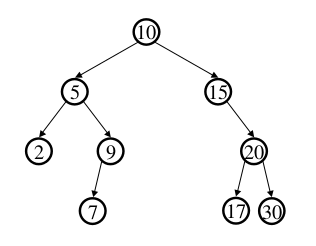
\includegraphics[width=\linewidth]{./Pictures/Inorder.png}
	\caption{Inorder Traversal: 2-5-7-9-10-15-17-20-30}
	\label{fig:??????}
	\end{center}
	\par\end{centering}
\end{figure}

%Why is logn good? There are roughly a billion websites on the internet -- if we could search them in logn time, it would take at most 30 steps to find an arbitray site.

%Strongly typed languages impose restrictions on what the data associated with a vertex must be.

%Traversals impose total order on the tree structure.

%Weighting edges on an undirected graph gives it a metric, or a fundamental notion of distance between points.

%Travelling salesman - NP Hard

%Structure - bijections between different choices of roots. Invariance of degree sequence between isomorphic graphs (isomorphisms preserve degree and edge structure). Invariance of distance between nodes.

%Trees are minimal connected subgraphs

%Laplace matrix Q of G
% qii = degree of vertex i
% qij = -1 if adjacent, 0 if not
% Delete any row and colum, det(Q) = number of distinct spanning trees
%
%



\end{document}
